% PopAgent System Walkthrough
% Comprehensive Technical Documentation for Presentation

\documentclass[11pt]{article}

\usepackage[utf8]{inputenc}
\usepackage[T1]{fontenc}
\usepackage{geometry}
\geometry{margin=1in}
\usepackage{hyperref}
\usepackage{booktabs}
\usepackage{amsmath}
\usepackage{amssymb}
\usepackage{graphicx}
\usepackage{xcolor}
\usepackage{listings}
\usepackage{algorithm}
\usepackage{algorithmic}
\usepackage{tcolorbox}
\usepackage{tikz}
\usetikzlibrary{shapes,arrows,positioning,fit,backgrounds}

% Custom colors
\definecolor{codeblue}{RGB}{0,102,204}
\definecolor{codegray}{RGB}{128,128,128}
\definecolor{codegreen}{RGB}{0,128,0}
\definecolor{backcolor}{RGB}{245,245,245}

% Code listing style
\lstset{
    backgroundcolor=\color{backcolor},
    basicstyle=\ttfamily\small,
    keywordstyle=\color{codeblue}\bfseries,
    commentstyle=\color{codegray},
    stringstyle=\color{codegreen},
    breaklines=true,
    frame=single,
    rulecolor=\color{gray},
}

% Custom box for key concepts
\newtcolorbox{keybox}[1][]{
    colback=blue!5,
    colframe=blue!50!black,
    title=#1,
    fonttitle=\bfseries
}

\newtcolorbox{questionbox}[1][]{
    colback=orange!5,
    colframe=orange!50!black,
    title=#1,
    fonttitle=\bfseries
}

\title{\Huge \textbf{PopAgent: System Architecture Walkthrough} \\[0.5em]
\Large Multi-Agent LLM Trading with Adaptive Method Selection}
\author{Technical Documentation for Presentation}
\date{\today}

\begin{document}

\maketitle

\tableofcontents
\newpage

%==============================================================================
\section{Executive Summary}
%==============================================================================

\begin{keybox}[What is PopAgent?]
PopAgent is a \textbf{multi-agent trading system} where agents \textbf{learn to SELECT which methods to use} from shared inventories, rather than being locked into fixed strategies. This creates a meta-learning system that discovers optimal method combinations through population-based continual learning.
\end{keybox}

\subsection{The One-Sentence Pitch}

\textit{``Instead of hand-designing trading agents, we let populations of agents learn which analytical methods work best for different market conditions, and share that knowledge across the population.''}

\subsection{Key Innovation}

\begin{center}
\begin{tabular}{|p{6cm}|p{6cm}|}
\hline
\textbf{Traditional Approach} & \textbf{PopAgent Approach} \\
\hline
Fixed agent strategies & Agents SELECT methods dynamically \\
Learn parameters (weights, thresholds) & Learn WHICH methods to use \\
Single best agent & Population discovers combinations \\
Static configurations & Adapts to market conditions \\
\hline
\end{tabular}
\end{center}

%==============================================================================
\section{System Overview}
%==============================================================================

\subsection{High-Level Architecture}

The system consists of four main layers:

\begin{enumerate}
    \item \textbf{Data Pipeline}: Fetches and processes price data (5 cryptocurrencies) and news
    \item \textbf{Agent Populations}: 4 roles $\times$ 5 agents each = 20 agents total
    \item \textbf{Learning Engine}: Thompson Sampling + Contextual Baselines + Multi-Step Returns
    \item \textbf{Execution}: Paper trading via Bybit Testnet
\end{enumerate}

\subsection{The Trading Pipeline}

Each trading iteration follows this flow:

\begin{center}
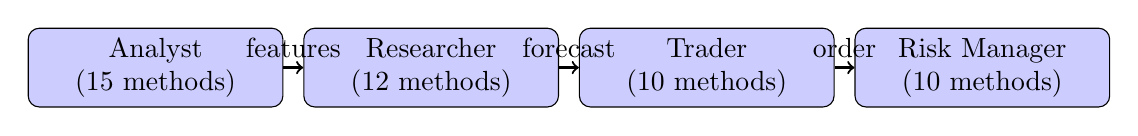
\begin{tikzpicture}[node distance=2cm, auto,
    block/.style={rectangle, draw, fill=blue!20, text width=3cm, text centered, rounded corners, minimum height=1cm},
    arrow/.style={->, thick}]
    
    \node[block] (analyst) {Analyst\\(15 methods)};
    \node[block, right of=analyst, node distance=3.5cm] (researcher) {Researcher\\(12 methods)};
    \node[block, right of=researcher, node distance=3.5cm] (trader) {Trader\\(10 methods)};
    \node[block, right of=trader, node distance=3.5cm] (risk) {Risk Manager\\(10 methods)};
    
    \draw[arrow] (analyst) -- node[above] {features} (researcher);
    \draw[arrow] (researcher) -- node[above] {forecast} (trader);
    \draw[arrow] (trader) -- node[above] {order} (risk);
    
\end{tikzpicture}
\end{center}

\textbf{Key insight}: Each role has an \textit{inventory} of methods (10-15), but each agent only \textit{selects 3} at a time. This creates selection pressure.

%==============================================================================
\section{The Four Agent Roles}
%==============================================================================

\subsection{Role 1: Analyst (Feature Engineering)}

\begin{keybox}[Analyst's Job]
Transform raw price data into meaningful features that signal trading opportunities.
\end{keybox}

\textbf{Input}: OHLCV price data (Open, High, Low, Close, Volume)

\textbf{Output}: Feature DataFrame with computed indicators

\textbf{Method Inventory (15 methods)}:

\begin{center}
\begin{tabular}{|l|l|p{6cm}|}
\hline
\textbf{Category} & \textbf{Methods} & \textbf{What They Compute} \\
\hline
Technical & RSI, MACD, Bollinger, ADX, Stochastic & Momentum, trend, volatility bands \\
Statistical & Autocorrelation, VolatilityClustering, MeanReversion, Cointegration & Statistical patterns \\
Decomposition & STL, Wavelet, Fourier & Time series decomposition \\
ML-Based & HMM\_Regime, Kalman, IsolationForest & Regime detection, filtering, anomalies \\
\hline
\end{tabular}
\end{center}

\textbf{Example}: An analyst might select \texttt{[RSI, HMM\_Regime, Wavelet]} based on learned preferences.

\subsection{Role 2: Researcher (Forecasting)}

\begin{keybox}[Researcher's Job]
Generate price forecasts with uncertainty quantification.
\end{keybox}

\textbf{Input}: Features from Analyst + historical prices

\textbf{Output}: Point forecast + confidence intervals

\textbf{Method Inventory (12 methods)}:

\begin{center}
\begin{tabular}{|l|l|p{6cm}|}
\hline
\textbf{Category} & \textbf{Methods} & \textbf{What They Do} \\
\hline
Statistical & ARIMA, ExpSmoothing, VAR, GARCH & Classical time series models \\
ML & RandomForest, GradientBoosting, LSTM, TemporalFusion & Machine learning forecasters \\
Uncertainty & Bootstrap, QuantileRegression, Bayesian, Conformal & Confidence interval methods \\
\hline
\end{tabular}
\end{center}

\textbf{Critical Output}: Not just a point forecast, but uncertainty bounds:
\begin{equation}
    \text{Forecast}: \hat{y}_{t+1} = 42{,}150 \pm 320 \text{ (95\% CI)}
\end{equation}

\subsection{Role 3: Trader (Order Generation)}

\begin{keybox}[Trader's Job]
Convert forecasts into concrete trading orders.
\end{keybox}

\textbf{Input}: Forecast + uncertainty from Researcher + news sentiment

\textbf{Output}: Trading order (direction, size, entry price, stop loss, take profit)

\textbf{Method Inventory (10 methods)}:

\begin{center}
\begin{tabular}{|l|l|p{6cm}|}
\hline
\textbf{Category} & \textbf{Methods} & \textbf{What They Control} \\
\hline
Execution & AggressiveMarket, PassiveLimit, TWAP, VWAP & How to execute (speed vs. cost) \\
Sizing & KellyCriterion, FixedFractional, VolatilityScaled & How much to trade \\
Entry & MomentumEntry, ContrarianEntry, BreakoutEntry & When to enter \\
\hline
\end{tabular}
\end{center}

\textbf{Example Order}:
\begin{lstlisting}
{
  "symbol": "BTCUSD.PERP",
  "side": "LONG",
  "position_size": 0.15,
  "leverage": 3,
  "entry_price": 42150,
  "stop_loss": 41500,
  "take_profit": 43200
}
\end{lstlisting}

\subsection{Role 4: Risk Manager (Validation)}

\begin{keybox}[Risk Manager's Job]
Validate orders against risk limits. Can PASS, SOFT\_FAIL (adjust), or HARD\_FAIL (block).
\end{keybox}

\textbf{Input}: Proposed order from Trader

\textbf{Output}: Verdict (PASS / SOFT\_FAIL / HARD\_FAIL) + adjusted order if needed

\textbf{Method Inventory (10 methods)}:

\begin{center}
\begin{tabular}{|l|l|p{6cm}|}
\hline
\textbf{Category} & \textbf{Methods} & \textbf{What They Check} \\
\hline
Position Limits & MaxLeverage, MaxPosition, Concentration & Size constraints \\
Loss Limits & MaxDrawdown, DailyStopLoss, TrailingStop & Loss protection \\
Risk Metrics & VaR, ExpectedShortfall & Statistical risk measures \\
Dynamic & VolatilityAdjusted, RegimeAware & Adaptive limits \\
\hline
\end{tabular}
\end{center}

\textbf{Verdict Logic}:
\begin{itemize}
    \item \textbf{PASS}: Order is within all limits, execute as-is
    \item \textbf{SOFT\_FAIL}: Order violates soft limits, adjust (reduce size/leverage)
    \item \textbf{HARD\_FAIL}: Order violates critical limits, block entirely
\end{itemize}

%==============================================================================
\section{The Method Selection System}
%==============================================================================

This is the \textbf{core innovation} of PopAgent.

\subsection{The Problem with Fixed Strategies}

Traditional approach:
\begin{lstlisting}[language=Python]
class TechnicalAnalyst:
    def analyze(self, prices):
        rsi = compute_rsi(prices)      # Always uses RSI
        macd = compute_macd(prices)    # Always uses MACD
        return rsi, macd               # Fixed methods
\end{lstlisting}

\textbf{Problem}: What if RSI works well in trending markets but poorly in ranging markets? The agent can't adapt.

\subsection{PopAgent's Solution: Method Selection}

Our approach:
\begin{lstlisting}[language=Python]
class MethodSelector:
    inventory = [RSI, MACD, Bollinger, HMM, Kalman, ...]  # 15 options
    preferences = {RSI: 0.8, MACD: 0.3, HMM: 1.2, ...}    # Learned
    
    def select_methods(self, context):
        # Sample from Beta distributions (Thompson Sampling)
        scores = {m: sample_beta(alpha[m], beta[m]) for m in inventory}
        selected = top_3(scores)  # Pick 3 methods
        return selected           # e.g., [RSI, HMM, Kalman]
\end{lstlisting}

\textbf{Key insight}: The agent learns WHICH methods to use, not just how to tune parameters.

\subsection{Why Inventory > Selection Creates Learning}

\begin{center}
\begin{tabular}{|c|c|c|}
\hline
\textbf{Inventory Size} & \textbf{Selection Size} & \textbf{Possible Combinations} \\
\hline
15 methods & 3 selected & $\binom{15}{3} = 455$ combinations \\
\hline
\end{tabular}
\end{center}

With 455 possible method combinations per role, agents must \textit{learn} which ones work. This is fundamentally different from parameter tuning.

%==============================================================================
\section{The Learning Algorithm}
%==============================================================================

\subsection{Overview: Three RL Enhancements}

We use three lightweight, theoretically-grounded RL techniques:

\begin{enumerate}
    \item \textbf{Thompson Sampling}: Bayesian exploration via Beta distributions
    \item \textbf{Contextual Baselines}: Per-regime reward normalization
    \item \textbf{Multi-Step Returns}: Temporal credit assignment
\end{enumerate}

\subsection{Enhancement 1: Thompson Sampling}

\begin{keybox}[Thompson Sampling Intuition]
Instead of always picking the method with highest expected reward (exploitation), sample from your uncertainty. Methods you're unsure about might randomly sample high, encouraging exploration.
\end{keybox}

\textbf{Mathematical Formulation}:

Each method $m$ has a Beta distribution representing our belief about its success probability:
\begin{equation}
    \theta_m \sim \text{Beta}(\alpha_m, \beta_m)
\end{equation}

where $\alpha_m$ = successes + 1, $\beta_m$ = failures + 1.

\textbf{Selection}: Sample from each distribution, pick top-$k$:
\begin{equation}
    S = \text{top-}k\left(\{\theta_m : m \in \mathcal{M}\}\right)
\end{equation}

\textbf{Update after reward $R$}:
\begin{equation}
    \alpha_m \leftarrow \alpha_m + \mathbb{1}[R > 0], \quad
    \beta_m \leftarrow \beta_m + \mathbb{1}[R \leq 0]
\end{equation}

\textbf{Example}:

\begin{center}
\begin{tabular}{|l|c|c|c|c|}
\hline
\textbf{Method} & $\alpha$ & $\beta$ & \textbf{Expected} & \textbf{Sample} \\
\hline
RSI & 15 & 5 & 0.75 & 0.82 \\
MACD & 8 & 12 & 0.40 & 0.35 \\
HMM & 3 & 2 & 0.60 & 0.71 \\
Kalman & 2 & 2 & 0.50 & 0.68 \\
\hline
\end{tabular}
\end{center}

In this sample, we'd select \texttt{[RSI, HMM, Kalman]} (top-3 samples), even though MACD has more data, because the samples favored the others.

\subsection{Enhancement 2: Contextual Baselines}

\begin{keybox}[Contextual Baseline Intuition]
A 2\% return means different things in different market conditions. In a bull market, it's average. In a bear market, it's exceptional. We need separate baselines per context.
\end{keybox}

\textbf{Context Discretization}:

We discretize market conditions into regimes:
\begin{equation}
    c = (\text{trend}, \text{volatility}, \text{regime})
\end{equation}

Example contexts:
\begin{itemize}
    \item \texttt{trend:bullish|vol:low|regime:normal}
    \item \texttt{trend:bearish|vol:high|regime:volatile}
\end{itemize}

\textbf{Per-Context Baseline}:
\begin{equation}
    \bar{R}_c = \frac{1}{n_c} \sum_{t: c_t = c} R_t
\end{equation}

\textbf{Contextual Advantage}:
\begin{equation}
    A = R - \bar{R}_c
\end{equation}

\textbf{Example}:

\begin{center}
\begin{tabular}{|l|c|c|c|}
\hline
\textbf{Context} & \textbf{Reward} & \textbf{Baseline} & \textbf{Advantage} \\
\hline
Bull market & +2\% & +2.5\% & -0.5\% (below average) \\
Bear market & +2\% & -0.5\% & +2.5\% (exceptional!) \\
\hline
\end{tabular}
\end{center}

The same reward gets different credit based on context.

\subsection{Enhancement 3: Multi-Step Returns}

\begin{keybox}[Multi-Step Return Intuition]
Some methods sacrifice short-term gains for long-term benefits. We need to credit methods for future outcomes, not just immediate rewards.
\end{keybox}

\textbf{$n$-Step Return}:
\begin{equation}
    G_t = R_t + \gamma R_{t+1} + \gamma^2 R_{t+2} + \ldots + \gamma^{n-1} R_{t+n-1}
\end{equation}

where $\gamma \in (0, 1)$ is the discount factor (we use $\gamma = 0.9$).

\textbf{Example}:

\begin{center}
\begin{tabular}{|l|c|c|c|c|}
\hline
\textbf{Method} & $R_0$ & $R_1$ & $R_2$ & $G$ (with $\gamma=0.9$) \\
\hline
Method A & +1\% & +0.5\% & +0.5\% & $1 + 0.45 + 0.41 = 1.86\%$ \\
Method B & -0.5\% & +3\% & +2\% & $-0.5 + 2.7 + 1.62 = 3.82\%$ \\
\hline
\end{tabular}
\end{center}

Method B looks bad initially but has better multi-step return.

%==============================================================================
\section{Population-Based Learning}
%==============================================================================

\subsection{Population Structure}

\begin{center}
\begin{tabular}{|l|c|l|}
\hline
\textbf{Role} & \textbf{Population Size} & \textbf{What Varies} \\
\hline
Analyst & 5 agents & Method selections, preferences \\
Researcher & 5 agents & Method selections, preferences \\
Trader & 5 agents & Method selections, preferences \\
Risk Manager & 5 agents & Method selections, preferences \\
\hline
\textbf{Total} & 20 agents & \\
\hline
\end{tabular}
\end{center}

\subsection{Pipeline Combinations}

In each iteration, we sample \textbf{pipeline combinations}:
\begin{equation}
    \text{Pipeline} = (\text{Analyst}_i, \text{Researcher}_j, \text{Trader}_k, \text{Risk}_l)
\end{equation}

With 5 agents per role: $5^4 = 625$ possible pipelines.

We sample 25 pipelines per iteration to keep computation tractable.

\subsection{Knowledge Transfer}

Every 10 iterations, we transfer knowledge from best to others:

\begin{algorithm}
\caption{Knowledge Transfer}
\begin{algorithmic}[1]
\FOR{each role $r \in \{\text{Analyst}, \text{Researcher}, \text{Trader}, \text{Risk}\}$}
    \STATE $a^* \leftarrow$ best agent in role $r$ (by average reward)
    \FOR{each agent $a \in$ role $r$, $a \neq a^*$}
        \STATE $\pi^a \leftarrow (1 - \tau) \cdot \pi^a + \tau \cdot \pi^{a^*}$ \COMMENT{Soft preference update}
        \STATE $\alpha^a \leftarrow (1 - \tau) \cdot \alpha^a + \tau \cdot \alpha^{a^*}$ \COMMENT{Thompson params}
    \ENDFOR
\ENDFOR
\end{algorithmic}
\end{algorithm}

Where $\tau = 0.1$ (transfer rate).

\textbf{Key insight}: We transfer \textit{preferences} (meta-knowledge about what works), not parameters of the methods themselves.

\subsection{Diversity Preservation}

To prevent population collapse (all agents converging to same methods):

\begin{enumerate}
    \item \textbf{Measure diversity}: Jaccard distance between agent selections
    \begin{equation}
        D = \frac{1}{\binom{N}{2}} \sum_{i < j} \left(1 - \frac{|S^i \cap S^j|}{|S^i \cup S^j|}\right)
    \end{equation}
    
    \item \textbf{If diversity $< 0.3$}: Boost exploration rate for non-best agents
    
    \item \textbf{Result}: Population maintains variety while still learning from best
\end{enumerate}

%==============================================================================
\section{Data Pipeline}
%==============================================================================

\subsection{Price Data}

\textbf{Source}: Bybit perpetual futures (4-hour candles)

\textbf{Assets}: 5 cryptocurrencies

\begin{center}
\begin{tabular}{|l|l|l|}
\hline
\textbf{Symbol} & \textbf{Name} & \textbf{Role} \\
\hline
BTC & Bitcoin & Primary benchmark \\
ETH & Ethereum & Smart contract platform \\
SOL & Solana & High-performance L1 \\
DOGE & Dogecoin & Retail sentiment indicator \\
XRP & Ripple & Payment-focused \\
\hline
\end{tabular}
\end{center}

\textbf{Features per asset}: OHLCV + Open Interest + Funding Rate + Long/Short Ratio

\subsection{Cross-Asset Features}

We compute 8 market-wide signals:

\begin{enumerate}
    \item \textbf{BTC Dominance}: BTC market cap relative to total
    \item \textbf{Altcoin Momentum}: Average momentum of non-BTC assets
    \item \textbf{ETH/BTC Ratio}: Risk-on/risk-off indicator
    \item \textbf{Cross OI Delta}: Aggregate open interest changes
    \item \textbf{Aggregate Funding}: Market-wide funding rate
    \item \textbf{Risk-On/Risk-Off}: Composite sentiment
    \item \textbf{Market Volatility}: Aggregate volatility measure
    \item \textbf{Cross-Correlation}: Asset correlation dynamics
\end{enumerate}

\subsection{News Pipeline}

\textbf{Source}: Bocha AI web search API

\textbf{Process}:
\begin{enumerate}
    \item Generate asset-specific queries (macro + micro news)
    \item Search via Bocha API
    \item Score source credibility (tier system)
    \item Enrich with LLM (sentiment, entities, impact)
    \item Aggregate into market digest
\end{enumerate}

%==============================================================================
\section{Project Structure}
%==============================================================================

\begin{lstlisting}[basicstyle=\ttfamily\footnotesize]
trading_agents/
|-- population/                # Core innovation
|   |-- selector.py           # MethodSelector class
|   |-- inventories.py        # 47 methods across 4 roles
|   |-- selector_workflow.py  # Learning loop
|   |-- transfer.py           # Knowledge transfer strategies
|   |-- diversity.py          # Diversity preservation
|   `-- scoring.py            # Shapley-based credit assignment
|
|-- agents/                   # Agent implementations
|   |-- analyst.py            # Feature engineering
|   |-- researcher.py         # Forecasting
|   |-- trader.py             # Order generation
|   |-- risk.py               # Risk validation
|   `-- admin.py              # Monitoring/reporting
|
|-- services/                 # Infrastructure
|   |-- llm.py                # LLM integration
|   |-- events.py             # Event bus
|   |-- notifications.py      # Alerts
|   `-- bybit_client.py       # Exchange API
|
`-- config/                   # Configuration
    `-- schemas.py            # Config dataclasses
\end{lstlisting}

%==============================================================================
\section{Anticipated Questions and Answers}
%==============================================================================

\begin{questionbox}[Q1: Why not use Deep RL (PPO, SAC)?]
\textbf{Answer}: Deep RL requires 100K+ samples, is prone to instability, and produces uninterpretable policies. Our bandit-based approach achieves competitive performance with 100$\times$ fewer samples while remaining fully interpretable. In finance, interpretability and sample efficiency are critical---traders need to understand why the system makes decisions.
\end{questionbox}

\begin{questionbox}[Q2: Why 5 agents per role? Why not more/fewer?]
\textbf{Answer}: 5 provides enough diversity for meaningful exploration while keeping computation tractable ($5^4 = 625$ pipeline combinations). Fewer agents risk premature convergence; more agents increase computational cost without proportional benefit due to diminishing returns.
\end{questionbox}

\begin{questionbox}[Q3: How do you handle the credit assignment problem?]
\textbf{Answer}: We use three approaches:
\begin{enumerate}
    \item \textbf{Individual scoring}: Each agent scored by average reward when participating
    \item \textbf{Pipeline scoring}: Consider how agents work together
    \item \textbf{Shapley values}: Fair credit attribution from cooperative game theory
\end{enumerate}
\end{questionbox}

\begin{questionbox}[Q4: What prevents all agents from converging to the same methods?]
\textbf{Answer}: Diversity preservation. We measure selection diversity via Jaccard distance. If diversity drops below 0.3, we boost exploration rates for non-best agents. Thompson Sampling also naturally maintains exploration through uncertainty.
\end{questionbox}

\begin{questionbox}[Q5: How does this compare to AutoML?]
\textbf{Answer}: Similar spirit but different focus. AutoML typically selects model architectures and hyperparameters once before training. We continuously adapt method selection during trading based on ongoing performance. It's more like online AutoML with population-based exploration.
\end{questionbox}

\begin{questionbox}[Q6: Can this overfit to recent market conditions?]
\textbf{Answer}: We mitigate overfitting through:
\begin{enumerate}
    \item \textbf{Contextual baselines}: Methods are evaluated relative to market regime
    \item \textbf{Population diversity}: Multiple agents prevent convergence to single strategy
    \item \textbf{Soft updates} ($\tau = 0.1$): Gradual preference transfer, not hard copying
    \item \textbf{Thompson Sampling}: Maintains exploration even as preferences develop
\end{enumerate}
\end{questionbox}

\begin{questionbox}[Q7: What's the computational cost?]
\textbf{Answer}: Very low compared to deep RL:
\begin{itemize}
    \item No neural network training
    \item Main cost is evaluating 25 pipelines per iteration
    \item Each pipeline: feature computation + forecast + order generation
    \item Runs on CPU, no GPU required
\end{itemize}
\end{questionbox}

\begin{questionbox}[Q8: How do you evaluate this system?]
\textbf{Answer}: Multiple metrics:
\begin{itemize}
    \item \textbf{Sharpe Ratio}: Risk-adjusted returns
    \item \textbf{Maximum Drawdown}: Worst peak-to-trough loss
    \item \textbf{Hit Rate}: Percentage of profitable trades
    \item \textbf{Calibration ECE}: Uncertainty quality
    \item \textbf{Learning curves}: Do preferences converge? Does performance improve?
\end{itemize}
\end{questionbox}

%==============================================================================
\section{Key Takeaways}
%==============================================================================

\begin{enumerate}
    \item \textbf{Method Selection as Meta-Learning}: Agents learn WHAT to use, not just parameters
    
    \item \textbf{Selection Pressure}: Inventory (15) $>$ Selection (3) creates meaningful choices
    
    \item \textbf{Lightweight RL}: Thompson Sampling + Contextual Baselines + Multi-Step Returns
    
    \item \textbf{Population Dynamics}: 20 agents explore, best knowledge transfers to others
    
    \item \textbf{Interpretability}: Clear preferences, no black-box neural networks
    
    \item \textbf{Sample Efficiency}: Works with limited financial data
\end{enumerate}

%==============================================================================
\section{References for Further Reading}
%==============================================================================

\begin{itemize}
    \item \textbf{Thompson Sampling}: Thompson (1933), ``On the likelihood that one unknown probability exceeds another''
    \item \textbf{Population-Based Training}: Jaderberg et al. (2017), ``Population Based Training of Neural Networks''
    \item \textbf{Shapley Values}: Shapley (1953), ``A value for n-person games''
    \item \textbf{Contextual Bandits}: Li et al. (2010), ``A Contextual-Bandit Approach to Personalized News Article Recommendation''
\end{itemize}

\end{document}

